% vim: set textwidth=78 autoindent:

\subsection{Plugin GPS }\label{label_plugingps}

% when the revision of a section has been finalized, 
% comment out the following line:
% \updatedisclaimer

\subsubsection{Cos'è un GPS?}\label{whatsgps}

GPS sta per Global Positioning System ed indica un sistema satellitare che permette a chiunque possegga un ricevitore GPS di trovare la propria posizione ovunque nel mondo.
Viene usato come ausilio nella navigazione, ad esempio in aereo, in barca o anche per semplici escursioni.
Il ricevitore GPS usa i segnali provenienti dai satelliti per calcolare la propria latitudine, longitudine and (talvolta) elevazione.
La maggior parte dei ricevitori ha anche la capacità di archiviare posizioni (note come \emph{waypoints}), sequenze di posizioni che costituiscono una rotta o \emph{route} pianificata e una traccia or \emph{track} dei propri movimenti nel tempo.
Waypoints, routes e tracks sono i tre elementi base dei dati GPS.
QGIS mostra i waypoints in layer di punti, mentre routes e tracks vengono mostrati in layer di linee.

\subsubsection{Caricare i dati GPS da un file}\label{label_loadgps}

Ci sono dozzine di diversi formati di file usati per archiviare dati GPS. Il formato usato da QGIS si chiama GPX (GPS eXchange format, formato di scambio GPS), che è un formato standard di interscambio che può contenere qualunque numero di waypoints, routes e tracks nello stesso file.

Per caricare un file GPX bisogna prima caricare il plugin.
\mainmenuopt{Plugins} > \dropmenuopttwo{mActionShowPluginManager}{Gestione Plugin...} > \checkbox{Strumenti GPS}. Quando questo plugin è caricato, un tasto indicante un piccolo dispositivo manuale GPS compare nella barra degli strumenti. Un file GPX di esempio è disponibile nel dataset:
\filename{/qgis\_sample\_data/gps/national\_monuments.gpx}. Vedere la Sezione~\ref{label_sampledata} per avere maggiori informazioni sui dati di esempio.

\begin{enumerate}
\item Cliccare l'icona \toolbtntwo{gps_importer}{strumenti GPS} e selezionare la tab \tab{Carica file GPX}.
\item \button{Sfoglia} la cartella \filename{qgis\_sample\_data/gps/},
selezionare il file GPX \filename{national\_monuments.gpx} e premere \button{Apri}.
\end{enumerate}

\begin{figure}[ht]
   \begin{center}
\caption{\label{gpxloader}La finestra di dialogo \emph{Strumenti GPS} \nixcaption}
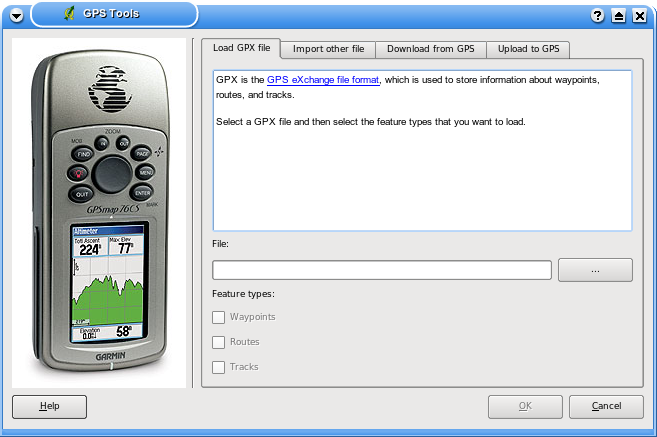
\includegraphics[clip=true, width=12cm]{loadgpx}
\end{center}
\end{figure}

Usare il pulsante Sfoglia \browsebutton per selezionare il file GPX, quindi selezionare con i checkbox i tipi di dati che si desidera caricare dal file GPX.
Ogni tipo di dato verrà caricato in uno layer separato quando si preme il pulsante \button{OK}.
Il file \filename{national\_monuments.gpx} include soltanto waypoints.

\subsubsection{GPSBabel}

Dato che QGIS usa file in formato GPX, è necessario un sistema per converti gli altri formati di file GPS in GPX.
Questo può essere fatto per molti formati usando il programma gratuito GPSBabel, che è disponibile a \url{http://www.gpsbabel.org}.
Questo programma può anche trasferire i dati GPS tra il computer e il dispositivo GPS. QGIS usa GPSBabel per fare queste cose, quindi si raccomanda di installare questo programma. Tuttavia, se si vuole solamente caricare dati GPS da file GPX, l'installazione non è necessaria.
È noto che la versione 1.2.3 di GPSBabel funziona con QGIS, ma non ci dovrebbero essere problemi anche con versioni successive.


\subsubsection{Importazione di dati GPS}

Per importare dati GPS da un file che non è in formato GPX, si può usare lo strumento \tab{Importa un altro file} nella finestra di dialogo Strumenti GPS.
Qui si selezione il file che si vuole importare, quali tipi di dati si vogliono importare da esso, dove deve essere archiviato il file convertito GPX e quale deve esser il nome del nuovo layer.

Quando si seleziona il file da importare, si deve anche specificare il formato di quel file usando il menu nelle finestra di dialogo di selezione file (vedere figura \ref{figure importdialog}). non tutti i formati supportano tutti e tre i tipi di dati, quindi per molti formati si potranno scegliere solamente uno o due tipi.

%\begin{figure}[ht]
%   \begin{center}
%\caption{\label{figure importdialog} Finestra di dialogo dello strumento di selezione del file da importare \nixcaption}
%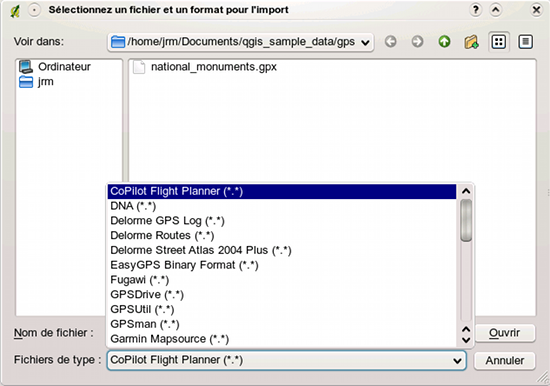
\includegraphics[clip=true, width=12cm]{importdialog}
%   \end{center}
%\end{figure}

\subsubsection{Scaricare dati GPS da un dispositivo}

QGIS può usare GPSBabel per scaricare i dati da un dispositivo GPS direttamente in layer vettoriali.
Per questo si usa lo strumento \tab{Download dal GPS} (vedere la Figura \ref{figure_download}), dove si seleziona il tipo di dispositivo GPS, La porta di comunicazione alla quale lo si è connesso, i tipi di dati che si vogliono scaricare, il nome del file GPX dove i dati devono essere archiviati e il nome del nuovo layer.

\begin{figure}[ht]
   \begin{center}
\caption{\label{figure_download}Lo strumento di download \nixcaption}
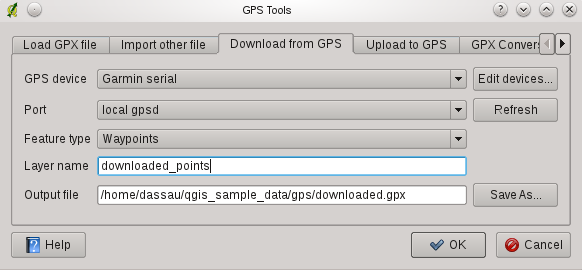
\includegraphics[clip=true, width=12cm]{download}
   \end{center}
\end{figure}


Il tipo di dispositivo che si seleziona nel menu dispositivi GPS determina il modo con cui GPSBabel cerca di comunicare con il dispositivo in questione. Se nessuno di questi tipi funziona con il dispositivo che si ha, si può creare un tipo nuovo (vedere sezione \ref{sec:Defining-new-device}).

la porta è un nome di file o un qualche altro nome che il sistema operativo usa nper riferirsi alla porta fisica del computer cui è connesso il dispositivo GPS.
\nix In Linux è qualcosa come /dev/ttyS0 or /dev/ttyS1 e in \win Windows è COM1 o COM2.

Quando si preme il pulsante \button{OK} i dati verranno scaricati dal dispositivo ed appariranno come layer in QGIS.

\subsubsection{Caricare dati GPS In un dispositivo}

Si può anche caricare dati direttamente da un layer vettoriale di QGIS in un dispositivo GPS, usando lo strumento \tab{Upload sul GPS}.
Il layer deve essere un layer GPX.
Per far questo semplicemente si seleziona il layer che si vuole caricare, il tipo di dispositivo GPS e la porta cui è connesso.
Come per lo strumento di download, bisogna specificare un nuov tipo di dispositivo se quello che si sta usando non è nella lista.

Questo strumento è molto utile insieme con le capacità di pubblicazione vettoriali di QGIS.
Si può caricare una mappa, creare alcuni waypoints e routes e poi caricarli ed utilizzarli nel proprio dispositivo GPS.

\subsubsection{\label{sec:Defining-new-device}Definizione di un nuovo dispositivo}

Ci sono molti tipi di dispositivi GPS.
Gli sviluppatori di QGIS non possono testarli tutti, quindi se se ne ha uno che non funziona con nessuno dei tipi elencati negli strumenti \tab{Download from GPS} and \tab{Upload to GPS} si può definire il proprio tipo di dispositivo per esso.
Questo può essere fatto usando l'editor di periferiche GPS, che si lancia premendo il pulsante \button{Modifica periferiche} nelle finestre di dialogo di download o di upload.

Per definire un nuovo dispositivo, semplicemente si preme il pulsante \button{Nuova periferica}, si sceglie un nome, un comando di download ed uno di upload per il dispositivo, e infine si preme il pulsante \button{Aggiorna periferiche}.
Il nome verrà elencato nel menu dei dispositivi nelle finestre di dialogo di upload e download, e può essere qualsiasi stringa.
Il comando di download è il comando usato per scaricare i dati dal dispositivo GPS al file GPX.
Questo probabilmente sarà un comando di GPSBabel, ma si può usare qualunque altra linea di comando che possa creare un file GPX.
QGIS sostituirà le parole chiave \usertext{\%type}, \usertext{\%in}, and \usertext{\%out} quando fa funzionare il comando.

\usertext{\%type} sarà sostituito da {}``\usertext{-w}'' se si stanno scaricando waypoints, {}``\usertext{-r}'' se si stanno scaricando routes e {}``\usertext{-t}'' se si stanno scaricando tracks.
Queste sono opzioni della linea di comando che dicono a GPSBabel quali tipi di dati scaricare.

\usertext{\%in} sarà sostituito dal nome della porta scelta nella finestra di dialogo di download e \usertext{\%out} sarà sostituito dal nome scelto per il file GPX in cui saranno archiviati i dati scaricati.
Così, se si crea un tipo di perfiferica con il comando di download {}``\usertext{gpsbabel \%type -i garmin -o gpx \%in \%out}'' (questo è in realtà il comando di dowload per il tipo di dispositivo predefinto \selectstring{GPS device:}{Garmin serial}) e lo si usa poi per scaricare waypoints dalla porta {}``\usertext{/dev/ttyS0}'' al file {}``\usertext{output.gpx}'', QGIS sostituirà le parole chiave ed eseguirà il comando {}``\usertext{gpsbabel -w -i garmin -o gpx /dev/ttyS0 output.gpx}''.

Il comando di upload è il comando che si usa per caricare dati sul disposiyivo GPS.
Si usano le stesse parole chiave, ma \usertext{\%in} è sostituita con il nome del file GPX per il layer che si sta caricando e \usertext{\%out} è sostituito dal nome della porta.

Per ulteriori informazioni su GPSBabel e per le opzioni disponibili per la sua lina di comando: \url{http://www.gpsbabel.org}

Una volta creata il nuovo tipo di perfierica, essa apparirà nella lista dei dispositivi per gli strumenti di download e upload.
